%
% exzess.tex
%
% (c) 2021 Prof Dr Andreas Müller, OST Ostschweizer Fachhochschule
%
\documentclass[tikz]{standalone}
\usepackage{times}
\usepackage{amsmath}
\usepackage{txfonts}
\usepackage[utf8]{inputenc}
\usepackage{graphics}
\usetikzlibrary{arrows,intersections,math}
\usepackage{ifthen}
\begin{document}

\newboolean{showgrid}
\setboolean{showgrid}{false}
\def\breite{7}
\def\hoehe{4}

\begin{tikzpicture}[>=latex,thick]

% Povray Bild
\begin{scope}
\clip (-6.3,-2.000) rectangle (6.3,2.000);
\node at (-4.225,0) {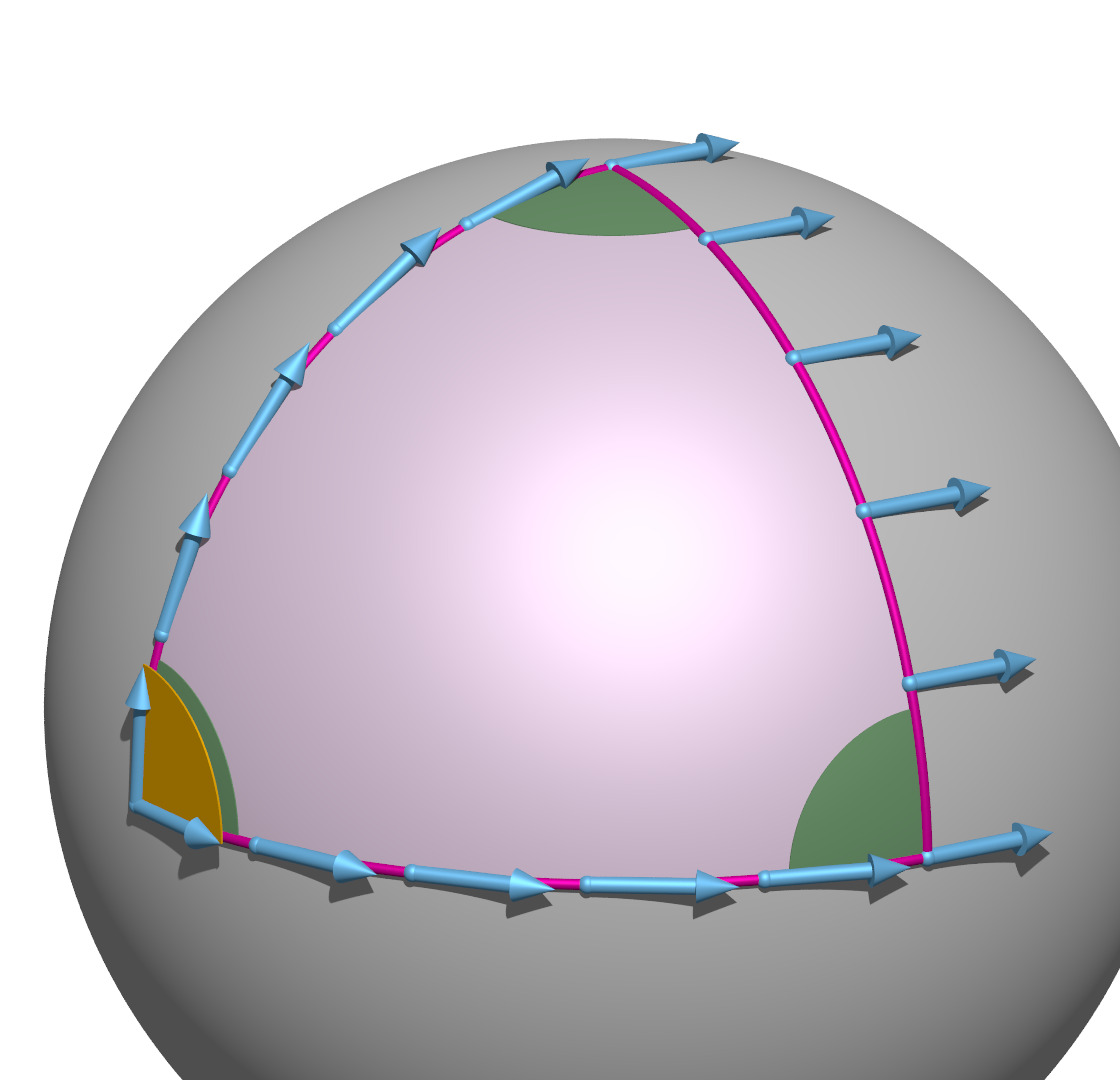
\includegraphics[width=4.15cm]{exzess0.jpg}};
\node at (0,0) {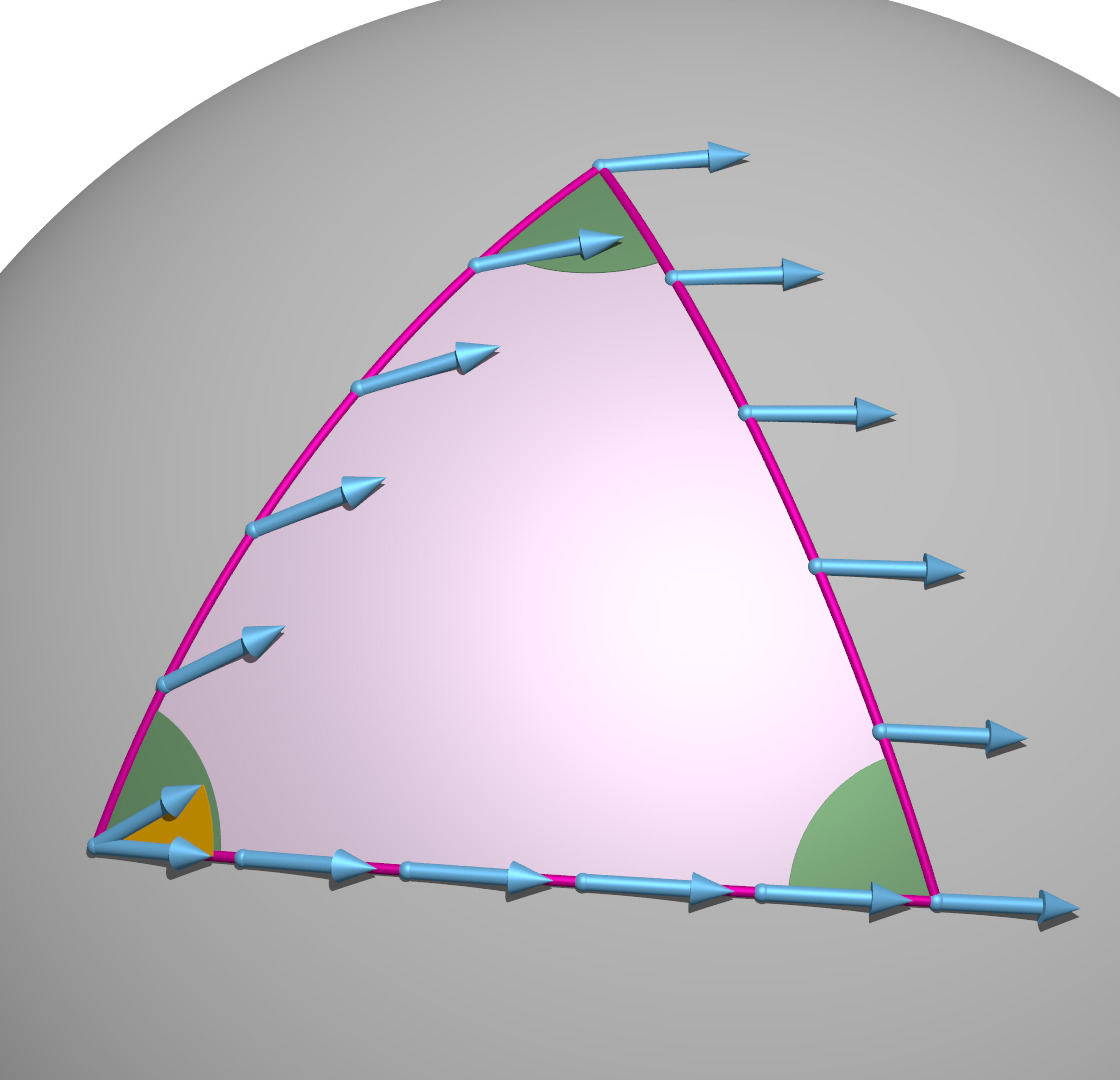
\includegraphics[width=4.15cm]{exzess1.jpg}};
\node at (4.225,0) {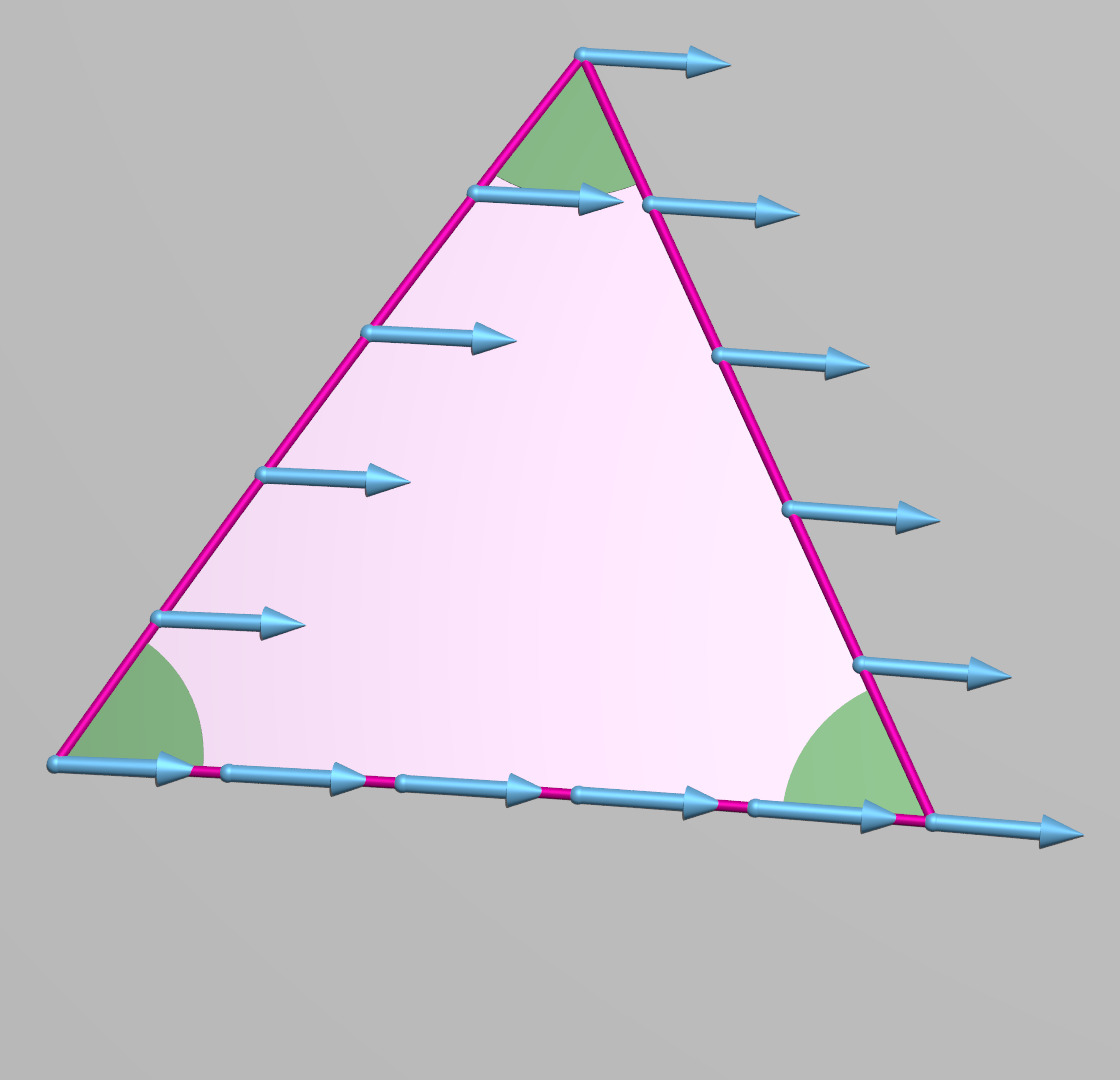
\includegraphics[width=4.15cm]{exzess2.jpg}};
\end{scope}

% Gitter
\ifthenelse{\boolean{showgrid}}{
\draw[step=0.1,line width=0.1pt] (-\breite,-\hoehe) grid (\breite, \hoehe);
\draw[step=0.5,line width=0.4pt] (-\breite,-\hoehe) grid (\breite, \hoehe);
\draw                            (-\breite,-\hoehe) grid (\breite, \hoehe);
\fill (0,0) circle[radius=0.05];
}{}

\node at (-5.9,-1.2) {$A$};
\node at (-5.3,-0.7) {$\alpha$};
\node at (-2.8,-1.4) {$B$};
\node at (-3.1,-1.0) {$\beta$};
\node at (-4,1.6) {$C$};
\node at (-4.1,1.2) {$\gamma$};
\node at (-4.3,-1.1) {$c$};
\node at (-3.3,0.2) {$a$};
\node at (-5.2,0.3) {$b$};

\begin{scope}[yshift=-0.2cm]
\node at (-1.8,-1.2) {$A$};
\node at (-1.1,-0.6) {$\alpha$};
\node at ( 1.4,-1.4) {$B$};
\node at (1.1,-0.9) {$\beta$};
\node at (0.15,1.8) {$C$};
\node[opacity=0.5] at (0.1,1.3) {$\gamma$};
\node at (-0.1,-0.85) {$c$};
\node at (0.7,0.2) {$a$};
\node at (-1.1,0.6) {$b$};
\end{scope}

\begin{scope}[xshift=-0.03cm,yshift=-0.4cm]
\node at (2.3,-1.05) {$A$};
\node at (2.7,-0.65) {$\alpha$};
\node at (5.65,-1.3) {$B$};
\node at (5.3,-0.8) {$\beta$};
\node at (4.3,2.0) {$C$};
\node at (4.275,1.45) {$\gamma$};
\node at (4.1,-1.15) {$c$};
\node at (4.8,0.3) {$a$};
\node at (3.2,0.6) {$b$};
\end{scope}

\end{tikzpicture}

\end{document}

